\documentclass[border=10pt]{standalone}
\usepackage{pgfplots}
\usepgfplotslibrary{fillbetween}
\pgfplotsset{every axis plot post/.append style =
  {samples=80, smooth, thick, black, mark=none} }
\begin{document}
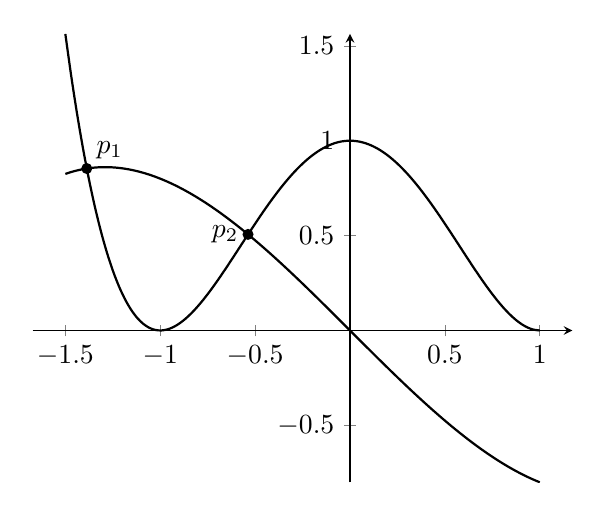
\begin{tikzpicture}
  \begin{axis}[axis lines = center, axis equal,
      domain = -1.5:1]
    \addplot[name path=cubic]   {x^3/5 - x};
    \addplot[name path=quartic] {(x^2-1)^2};
    \fill[name intersections = {of=cubic and quartic,
     name=p}]
      (p-1) circle (2pt) node [above right] {$p_1$}
      (p-2) circle (2pt) node [left]        {$p_2$};
  \end{axis}
\end{tikzpicture}
\end{document}
